\RequirePackage{plautopatch}
\documentclass[a4paper,10pt]{article}
\usepackage{amsmath}
\usepackage{siunitx}
\usepackage{graphicx}
\usepackage{csvsimple}
\usepackage{url}

\title{Title on the Experiment}
\author{Yamaguchi Kanon}
\date{Conducted on 2025-00-00}

\begin{document} 

    \maketitle

    \section{原理}
    
    神のみぞ知る真の値$X$と，測定データ${x_i}$の差${x_i -X}$を誤差という．誤差の平均を標準偏差$\sigma$という．
    \begin{align}
        \sigma = \sqrt{\frac{1}{N} \sum_{i=1}^{N}(x_i - X)^2}
    \end{align}
    これは$\left| \sum_{i\neq j}(x_i -X)(x_j - X) \right| << N$ならば，
    \begin{align}
        \sigma = \sqrt{\frac{1}{N-1} \sum_{i=1}^{N}(x_i - \langle x\rangle)^2}
    \end{align}
    また，平均$\langle x\rangle$の標準偏差が$sqrt{N}$に反比例すること（大数の法則）を認めると，
    \begin{align}
        \Delta \langle x\rangle = \frac{\Delta x}{\sqrt{N}} = \sqrt{\frac{1}{N(N-1)} \sum_{i=1}^{N}(x_i - \langle x\rangle)^2}
    \end{align}
    
    また，標本数$N$が十分でない場合，$\chi$-分布を考えればよい．

    \section{実験方法}
    図\ref{fg:figure}のように装置を組む．
    \begin{figure}[htbp]
        \centering
        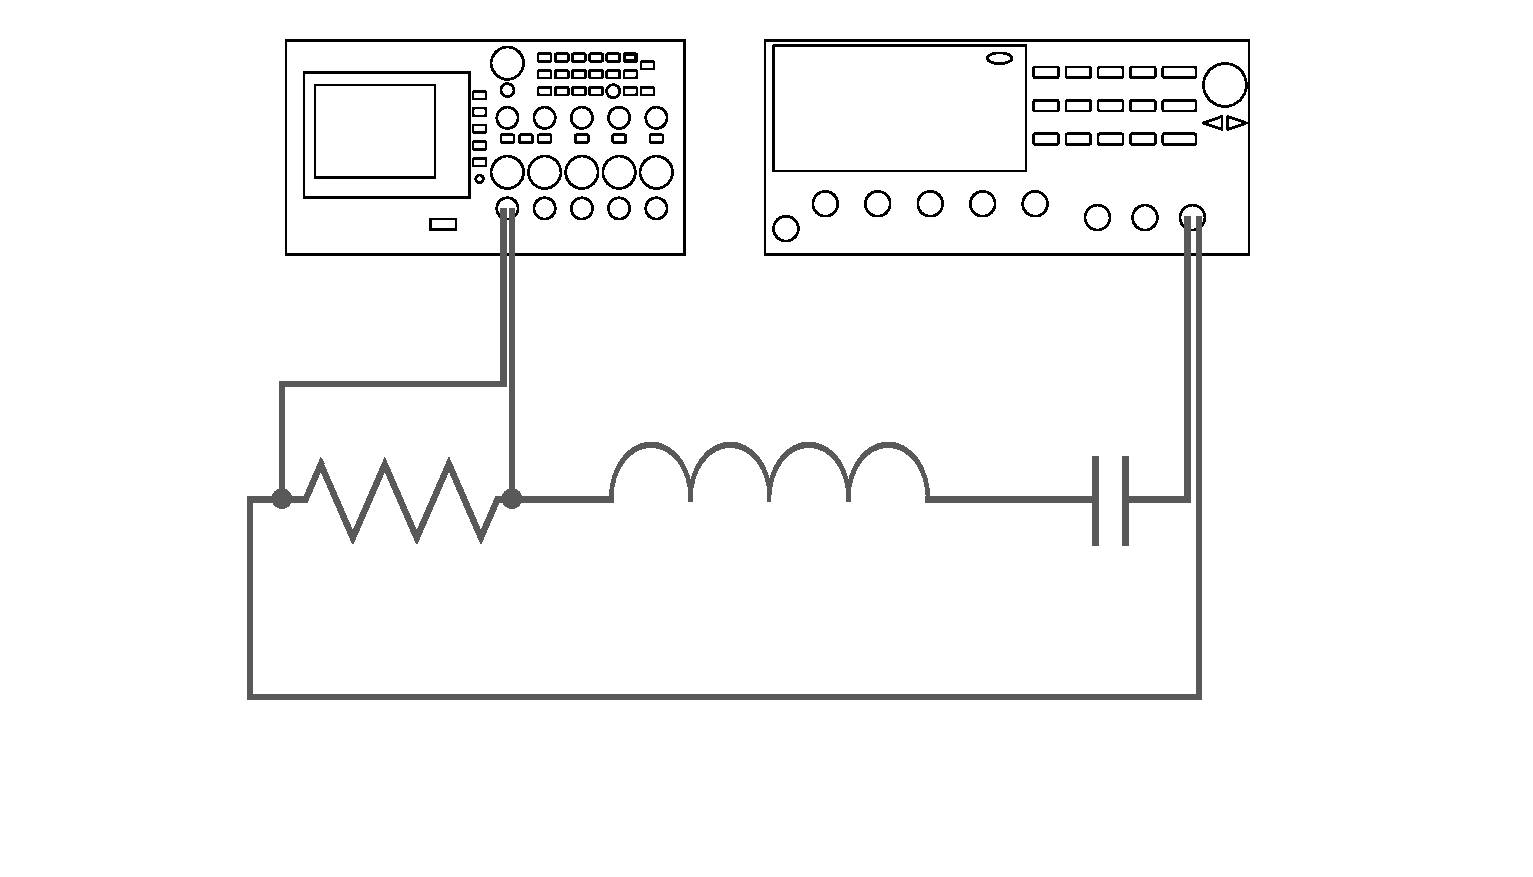
\includegraphics[width=8cm]{material/sample.eps}
        \caption{図の名前}
        \label{fg:figure}
    \end{figure}
    この際，あれこれのことに注意してくみ上げた．

    \subsection{使用機器}

    使用した機器は表\ref{tb:device}に示す．
    \begin{table}[htbp]
        \centering
        \caption{使用機器}
        \label{tb:device}
        \begin{tabular}{lrlll}
            \hline
            機器 & 個数 & 製造会社 & 型番号 & 備考\\ \hline
            \csvreader[late after line=\\]{material/device.csv}
            {name=\name,num=\num,co=\co,model=\model,note=\note}
            {\name & \num 個 & \co & \model & \note}
            \hline
        \end{tabular}
    \end{table}
    \section{結果}
    \section{考察}
    \begin{thebibliography}{99}
        \bibitem{citekey} Title, Company, \url{example.com}, Date.
    \end{thebibliography}
\end{document}